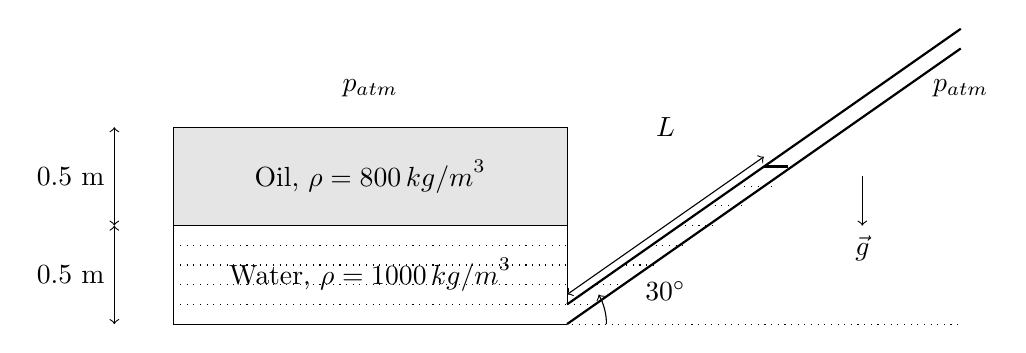
\begin{tikzpicture}[scale=2.5] 

\def\oilheight{0.5}
\def\waterheight{0.5}
\def\totalheight{\oilheight+\waterheight}
\def\angle{30}
\def\length{3}

\fill[gray!20] (0,0) rectangle (2,\oilheight);
\draw (0,0)--(2,0);
\draw (0,-0.5)--(2,-0.5);
\draw (0,0.5)--(2,0.5);
\draw (0,-0.5)--(0,0.5);
\draw (2,-0.4)--(2,0.5);
\node at (1,\oilheight/2) {Oil, $\rho = 800 \, \text{kg/m}^3$};
\node at (1,-\waterheight/2) {Water, $\rho = 1000 \, \text{kg/m}^3$};
\draw[<->] (-0.3,0) -- (-0.3,\oilheight) node[midway,left] {0.5 m};
\draw[<->] (-0.3,-\waterheight) -- (-0.3,0) node[midway,left] {0.5 m};
\node at (1,\totalheight-0.30) {$p_{\text{atm}}$};
\node at (4,\totalheight-0.30) {$p_{\text{atm}}$};
\draw[thick](3,0.3)--(3.12,0.3);
\draw[dotted](0,-0.5)--(4,-0.5);
\draw[thick](2,-0.50)--(4,0.9);
\draw[thick](2,-0.4)--(4,1);
\draw[<->](2,-0.35)--(3,0.35);
\draw[->] (2.2,-\waterheight+0) arc[start angle=0, end angle=30, radius=0.3];
\node at (2.5,-\waterheight+0.17) {$30^\circ$};
\node at (2.5,0.5) {$L$};
\draw[dotted] (0,-0.4)--(2,-0.4);
\draw[dotted] (0,-0.3)--(2,-0.3);
\draw[dotted] (0,-0.2)--(2,-0.2);
\draw[dotted] (0,-0.1)--(2,-0.1);
\draw[dotted] (2,-0.4)--(2.15,-0.4);
\draw[dotted] (2.15,-0.3)--(2.3,-0.3);
\draw[dotted] (2.30,-0.2)--(2.45,-0.2);
\draw[dotted] (2.45,-0.1)--(2.6,-0.1);
\draw[dotted] (2.6,0)--(2.75,0);
\draw[dotted] (2.75,0.1)--(2.9,0.1);
\draw[dotted] (2.9,0.2)--(3.05,0.2);
\draw[->] (3.5,0.25) -- (3.5,0) node[below] {$\vec{g}$};
\end{tikzpicture}
